\chapter{Multivariate Distributions}

Many problems involve several random variables at once: the number of each blood type in
a sample, the height and weight of a person, the scores on two tests. This chapter treats
discrete random variables jointly (the continuous case works the same way with integrals
replacing sums).

\section{Joint and marginal probability functions}

\begin{definition}[Joint p.f.]
The \emph{joint probability function} of discrete r.v.s $X$ and $Y$ is
\[
  f(x,y) = P(X = x, Y = y) = P(\{X=x\}\cap\{Y=y\}).
\]
It satisfies $f(x,y)\ge 0$ and $\sum_x\sum_y f(x,y) = 1$. For any set $A$ of pairs,
$P((X,Y)\in A) = \sum_{(x,y)\in A} f(x,y)$. The definition extends to $X_1,\dots,X_n$.
\end{definition}

\begin{definition}[Marginal p.f.]
The \emph{marginal} probability functions are
\[
  f_1(x) = P(X = x) = \sum_y f(x,y), \qquad f_2(y) = P(Y=y) = \sum_x f(x,y).
\]
\end{definition}

In a table of $f(x,y)$, the marginals are the row and column totals (written in the
``margins'').

\begin{example}[Running example]
Let $X\in\{0,1,2\}$ and $Y\in\{0,1\}$ have joint p.f.

\begin{center}
\begin{tabular}{c|ccc|c}
$f(x,y)$ & $x=0$ & $x=1$ & $x=2$ & $f_2(y)$ \\
\hline
$y=0$ & $0.1$ & $0.2$ & $0.1$ & $0.4$ \\
$y=1$ & $0.2$ & $0.1$ & $0.3$ & $0.6$ \\
\hline
$f_1(x)$ & $0.3$ & $0.3$ & $0.4$ & $1$ \\
\end{tabular}
\end{center}

Then, for example, $P(X > Y) = f(1,0) + f(2,0) + f(2,1) = 0.2 + 0.1 + 0.3 = 0.6$ and
$P(X+Y = 2) = f(2,0) + f(1,1) = 0.2$.
\end{example}

\begin{center}
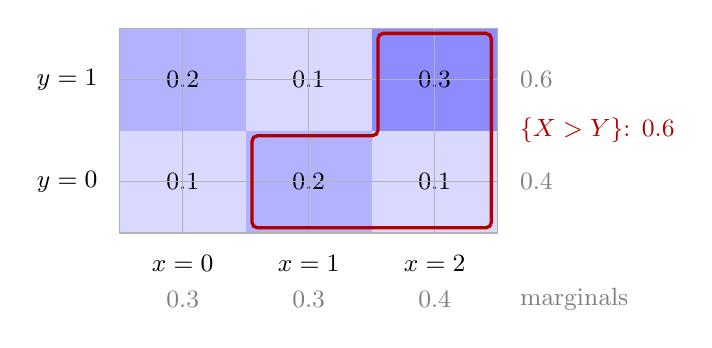
\begin{tikzpicture}[x=1.6cm, y=1.3cm, every node/.style={font=\small}]
  \fill[blue!15] (-0.5,-0.5) rectangle (0.5,0.5);
  \node at (0,0) {$0.1$};
  \fill[blue!30] (0.5,-0.5) rectangle (1.5,0.5);
  \node at (1,0) {$0.2$};
  \fill[blue!15] (1.5,-0.5) rectangle (2.5,0.5);
  \node at (2,0) {$0.1$};
  \fill[blue!30] (-0.5,0.5) rectangle (0.5,1.5);
  \node at (0,1) {$0.2$};
  \fill[blue!15] (0.5,0.5) rectangle (1.5,1.5);
  \node at (1,1) {$0.1$};
  \fill[blue!45] (1.5,0.5) rectangle (2.5,1.5);
  \node at (2,1) {$0.3$};
  \draw[gray!60] (-0.5,-0.5) grid[xstep=1, ystep=1] (2.5,1.5);
  \draw[gray!60] (-0.5,-0.5) rectangle (2.5,1.5);
  \draw[very thick, red!70!black, rounded corners=2pt] (0.55,-0.45) -- (2.45,-0.45) -- (2.45,1.45) -- (1.55,1.45) -- (1.55,0.45) -- (0.55,0.45) -- cycle;
  \foreach \x in {0,1,2} \node at (\x,-0.8) {$x=\x$};
  \foreach \y in {0,1} \node[anchor=east] at (-0.6,\y) {$y=\y$};
  \node[text=gray] at (0,-1.15) {$0.3$}; \node[text=gray] at (1,-1.15) {$0.3$}; \node[text=gray] at (2,-1.15) {$0.4$};
  \node[text=gray, anchor=west] at (2.6,0) {$0.4$}; \node[text=gray, anchor=west] at (2.6,1) {$0.6$};
  \node[text=gray, anchor=west] at (2.6,-1.15) {marginals};
  \node[text=red!70!black, anchor=west] at (2.6,0.5) {$\{X>Y\}$: $0.6$};
\end{tikzpicture}
\end{center}
Darker cells carry more probability; the outlined cells make up the event $\{X > Y\}$, and
the grey numbers are the row and column totals.

\section{Independent random variables}

\begin{definition}[Independence]
$X$ and $Y$ are \emph{independent} if
\[
  f(x,y) = f_1(x)f_2(y) \quad\text{for \emph{all} } x, y.
\]
Equivalently, the events $\{X = x\}$ and $\{Y=y\}$ are independent for every pair
$(x,y)$. $X_1,\dots,X_n$ are independent if
$f(x_1,\dots,x_n) = f_1(x_1)\cdots f_n(x_n)$ for all values.
\end{definition}

To show dependence, a single pair with $f(x,y)\ne f_1(x)f_2(y)$ suffices. A quick test:
if the range of $(X,Y)$ is not a ``rectangle'' (some $f(x,y) = 0$ while
$f_1(x), f_2(y) > 0$), then $X$, $Y$ are dependent.

\begin{example}
In the running example, $f(0,0) = 0.1$ but $f_1(0)f_2(0) = 0.3\times0.4 = 0.12$, so $X$
and $Y$ are \emph{not} independent.
\end{example}

\section{Conditional distributions}

\begin{definition}[Conditional p.f.]
The \emph{conditional probability function of $X$ given $Y = y$} is
\[
  f_1(x\given y) = P(X = x\given Y = y) = \frac{f(x,y)}{f_2(y)}, \qquad f_2(y) > 0.
\]
\end{definition}

For fixed $y$ this is a genuine p.f.\ in $x$. $X$ and $Y$ are independent iff
$f_1(x\given y) = f_1(x)$ for all $x$, $y$.

\begin{example}
In the running example, given $Y=1$:
$f_1(0\given1) = 0.2/0.6 = 1/3$, $f_1(1\given1) = 0.1/0.6 = 1/6$,
$f_1(2\given1) = 0.3/0.6 = 1/2$, which differs from the marginal $(0.3, 0.3, 0.4)$.
\end{example}

\begin{center}
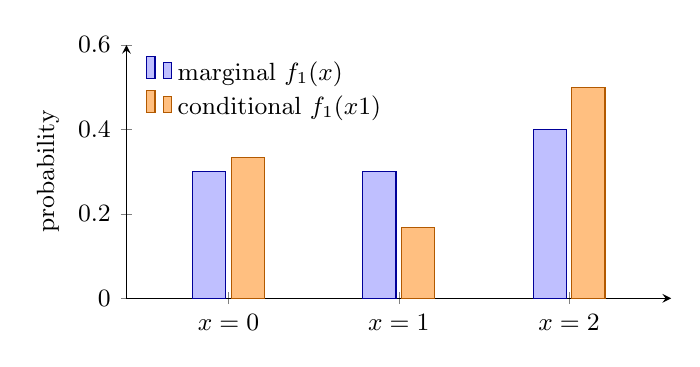
\begin{tikzpicture}
\begin{axis}[width=8.5cm, height=4.8cm, ybar, bar width=12pt, ymin=0, ymax=0.6,
    xtick={0,1,2}, xticklabels={$x=0$,$x=1$,$x=2$}, ylabel={probability}, tick label style={font=\small}, label style={font=\small}, axis lines=left, scaled y ticks=false, yticklabel style={/pgf/number format/fixed},
    enlarge x limits=0.3, legend style={font=\small, draw=none, at={(0.02,0.98)}, anchor=north west},
    legend cell align=left]
  \addplot[fill=blue!25, draw=blue!60!black] coordinates {(0,0.3) (1,0.3) (2,0.4)};
  \addplot[fill=orange!50, draw=orange!70!black] coordinates {(0,0.3333) (1,0.1667) (2,0.5)};
  \legend{marginal $f_1(x)$, conditional $f_1(x\given 1)$}
\end{axis}
\end{tikzpicture}
\end{center}

\subsection{Functions of random variables}

To find the distribution of $T = g(X,Y)$, add up $f(x,y)$ over the pairs with
$g(x,y) = t$. For sums of independent non-negative integer r.v.s this is a
\emph{convolution}: $P(X+Y = t) = \sum_{x=0}^t f_1(x)f_2(t-x)$.

\begin{theorem}[Sums of independent Poissons]
If $X\sim\Poi(\mu_1)$ and $Y\sim\Poi(\mu_2)$ are independent, then
$X+Y\sim\Poi(\mu_1+\mu_2)$, and the conditional distribution of $X$ given $X+Y = n$ is
$\Bin\left(n, \frac{\mu_1}{\mu_1+\mu_2}\right)$.
\end{theorem}

\begin{proof}
\[
  P(X+Y = t) = \sum_{x=0}^t \frac{e^{-\mu_1}\mu_1^x}{x!}\cdot\frac{e^{-\mu_2}\mu_2^{t-x}}{(t-x)!}
  = \frac{e^{-(\mu_1+\mu_2)}}{t!}\sum_{x=0}^t\binom tx\mu_1^x\mu_2^{t-x}
  = \frac{e^{-(\mu_1+\mu_2)}(\mu_1+\mu_2)^t}{t!}.
\]
Then $P(X = x\given X+Y = n) = P(X=x)P(Y=n-x)/P(X+Y=n)$, which simplifies to
$\binom nx \left(\frac{\mu_1}{\mu_1+\mu_2}\right)^x\left(\frac{\mu_2}{\mu_1+\mu_2}\right)^{n-x}$.
\end{proof}

Similarly, if $X\sim\Bin(n,p)$ and $Y\sim\Bin(m,p)$ are independent (same $p$), then
$X+Y\sim\Bin(n+m,p)$.

\section{The multinomial distribution}

The multinomial generalises the binomial to more than two outcome categories.

\textbf{Setup.} Each of $n$ independent trials results in exactly one of $k$ types, with
probabilities $p_1,\dots,p_k$ ($\sum p_i = 1$). Let $X_i$ be the number of trials of type
$i$.

\begin{theorem}[Multinomial p.f.]
\[
  f(x_1,\dots,x_k) = \frac{n!}{x_1!\,x_2!\cdots x_k!}p_1^{x_1}p_2^{x_2}\cdots p_k^{x_k},
  \qquad x_i\ge 0,\ \sum_i x_i = n.
\]
We write $(X_1,\dots,X_k)\sim\Mult(n; p_1,\dots,p_k)$.
\end{theorem}

\begin{proof}
Each particular sequence with $x_i$ outcomes of type $i$ has probability
$\prod p_i^{x_i}$, and the number of such sequences is the multinomial coefficient
(arrangements with repeats, Chapter 3).
\end{proof}

The $X_i$ are \emph{dependent} (they must sum to $n$). Each marginal is binomial:
$X_i\sim\Bin(n,p_i)$, since each trial is either type $i$ or not. Likewise sums of
categories are binomial, e.g.\ $X_1 + X_2\sim\Bin(n, p_1+p_2)$.

\begin{example}[Blood types]
In a population, blood types O, A, B, AB occur with probabilities $0.45$, $0.40$, $0.11$,
$0.04$. In a random sample of $10$ people,
\[
  P(5\text{ O}, 3\text{ A}, 2\text{ B}, 0\text{ AB}) = \frac{10!}{5!\,3!\,2!\,0!}
  (0.45)^5(0.40)^3(0.11)^2(0.04)^0 \approx 0.0360.
\]
\end{example}

\begin{example}[Dice]
A fair die is rolled $10$ times. The probability of exactly three $1$'s, two $2$'s and
five other faces is
\[
  \frac{10!}{3!\,2!\,5!}\left(\frac16\right)^3\left(\frac16\right)^2\left(\frac46\right)^5
  = 2520\cdot\frac{32}{1\,889\,568} \approx 0.0427.
\]
\end{example}

\section{Expectation of functions of several random variables}

\begin{definition}
$\E[g(X,Y)] = \sum_x\sum_y g(x,y)f(x,y)$.
\end{definition}

\begin{theorem}[Properties]
\begin{enumerate}
  \item $\E[aX + bY] = a\E(X) + b\E(Y)$ for any $X$, $Y$ (independent or not).
  \item If $X$ and $Y$ are independent, then $\E[g(X)h(Y)] = \E[g(X)]\E[h(Y)]$; in
        particular $\E(XY) = \E(X)\E(Y)$.
\end{enumerate}
\end{theorem}

\begin{proof}
(1) $\sum\sum(ax+by)f(x,y) = a\sum_x x f_1(x) + b\sum_y yf_2(y)$, using the marginals.
(2) With $f(x,y) = f_1(x)f_2(y)$, the double sum factors as
$\left(\sum_x g(x)f_1(x)\right)\left(\sum_y h(y)f_2(y)\right)$.
\end{proof}

\section{Covariance and correlation}

\begin{definition}[Covariance]
\[
  \Cov(X,Y) = \E[(X-\mu_X)(Y-\mu_Y)] = \E(XY) - \E(X)\E(Y).
\]
\end{definition}

Covariance is positive when large values of $X$ tend to go with large values of $Y$, and
negative when large $X$ goes with small $Y$.

\begin{theorem}[Properties of covariance]
\begin{enumerate}
  \item $\Cov(X,X) = \Var(X)$ and $\Cov(X,Y) = \Cov(Y,X)$.
  \item $\Cov(aX+b, cY+d) = ac\Cov(X,Y)$.
  \item $\Cov(X, Y+W) = \Cov(X,Y) + \Cov(X,W)$ (bilinearity).
  \item If $X$ and $Y$ are independent, $\Cov(X,Y) = 0$.
\end{enumerate}
\end{theorem}

\begin{important}[Zero covariance does not imply independence]
Let $X$ be uniform on $\{-1,0,1\}$ and $Y = X^2$. Then $\E(X) = 0$ and
$\E(XY) = \E(X^3) = 0$, so $\Cov(X,Y) = 0$; but $Y$ is a function of $X$, and indeed
$P(X=0,Y=1) = 0 \ne P(X=0)P(Y=1) = \frac13\cdot\frac23$.
\end{important}

\begin{definition}[Correlation]
\[
  \rho = \Corr(X,Y) = \frac{\Cov(X,Y)}{\SD(X)\SD(Y)}.
\]
\end{definition}


\begin{center}
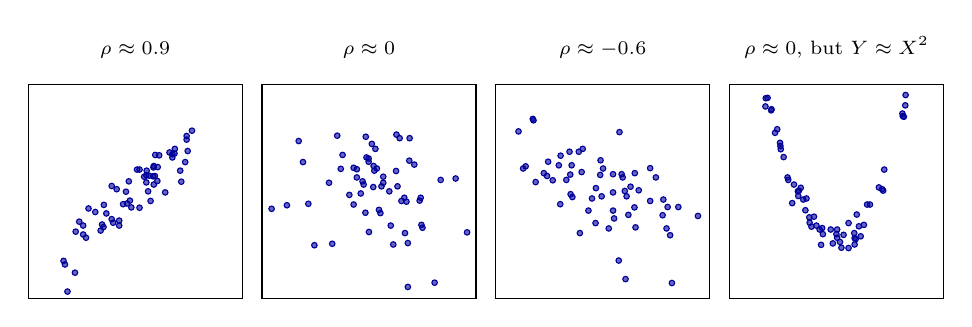
\begin{tikzpicture}
\begin{axis}[name=p0, width=4.3cm, height=4.3cm, xmin=-3, xmax=3, ymin=-3, ymax=3,
    xtick=\empty, ytick=\empty, title={$\rho\approx 0.9$}, title style={font=\scriptsize}]
  \addplot[only marks, mark=*, mark size=1pt, blue!60!black, fill opacity=0.6] coordinates {(-0.26,-0.01) (-0.23,-0.34) (-0.93,-0.93) (1.11,1.19) (1.04,1.04) (0.39,0.44) (-1.67,-1.13) (0.51,0.67) (-1.69,-2.28) (-0.89,-1.00) (0.31,0.25) (0.52,0.19) (0.31,0.45) (-0.66,0.15) (0.56,1.02) (-0.62,-0.88) (-0.34,-0.36) (0.63,0.68) (-0.45,-0.82) (-0.52,0.06) (-0.81,-0.62) (0.43,-0.27) (0.05,0.61) (-2.01,-1.95) (-0.11,-0.45) (0.50,0.42) (-1.46,-0.96) (0.67,1.01) (1.44,1.45) (0.12,-0.46) (0.62,0.29) (-0.45,-0.96) (-0.97,-1.10) (1.29,0.27) (-1.46,-1.21) (1.44,1.55) (-1.90,-2.81) (0.36,0.00) (-1.12,-0.58) (1.10,1.06) (0.25,0.41) (1.59,1.70) (0.52,0.71) (-1.57,-0.85) (0.96,1.09) (-1.97,-2.05) (0.84,-0.03) (-0.18,0.28) (-1.31,-0.48) (0.55,0.43) (0.32,0.58) (0.12,0.61) (-0.66,-0.78) (1.04,0.95) (-0.88,-0.38) (1.47,1.13) (-1.38,-1.30) (-0.15,-0.26) (1.40,0.82) (1.26,0.58)};
\end{axis}
\begin{axis}[name=p1, at={(p0.east)}, anchor=west, xshift=0.25cm, width=4.3cm, height=4.3cm, xmin=-3, xmax=3, ymin=-3, ymax=3,
    xtick=\empty, ytick=\empty, title={$\rho\approx 0$}, title style={font=\scriptsize}]
  \addplot[only marks, mark=*, mark size=1pt, blue!60!black, fill opacity=0.6] coordinates {(-0.79,0.63) (1.13,0.86) (0.35,0.14) (0.15,0.58) (-0.18,0.28) (0.57,0.00) (0.76,0.57) (2.01,0.32) (-0.43,-0.37) (-0.01,0.92) (-0.34,0.39) (1.84,-2.56) (-1.12,0.24) (0.40,0.24) (-0.43,0.66) (0.28,-0.52) (2.43,0.36) (-0.55,-0.10) (-0.23,-0.06) (-2.73,-0.49) (1.01,-1.17) (-0.07,0.95) (0.86,1.49) (-1.70,-0.35) (-0.34,0.62) (1.09,-2.68) (1.09,-1.45) (0.68,-1.49) (0.18,1.19) (-0.15,0.19) (0.80,0.14) (-0.09,1.53) (1.05,-0.29) (2.75,-1.15) (0.91,-0.27) (0.13,0.71) (0.22,0.64) (-1.53,-1.51) (0.61,-0.96) (-1.03,-1.47) (1.27,0.75) (1.47,-0.94) (0.00,-1.14) (0.77,1.59) (-0.89,1.56) (0.99,-0.18) (-1.97,1.41) (-0.10,-0.60) (0.40,0.41) (1.50,-1.02) (1.14,1.49) (1.45,-0.18) (-0.74,1.02) (0.12,0.12) (1.42,-0.26) (-2.30,-0.39) (-1.85,0.82) (0.32,-0.61) (-0.01,0.83) (0.08,1.33)};
\end{axis}
\begin{axis}[name=p2, at={(p1.east)}, anchor=west, xshift=0.25cm, width=4.3cm, height=4.3cm, xmin=-3, xmax=3, ymin=-3, ymax=3,
    xtick=\empty, ytick=\empty, title={$\rho\approx -0.6$}, title style={font=\scriptsize}]
  \addplot[only marks, mark=*, mark size=1pt, blue!60!black, fill opacity=0.6] coordinates {(-0.06,0.87) (1.49,0.39) (-0.67,1.11) (-1.88,0.26) (-1.96,2.03) (-1.23,0.73) (-0.19,0.09) (-0.59,0.54) (1.79,-1.04) (0.53,0.48) (-0.20,-0.89) (-0.56,1.19) (-1.65,0.51) (1.01,0.03) (0.01,0.64) (0.17,-1.04) (-1.56,0.43) (0.92,-1.01) (-0.90,-0.08) (-1.53,0.83) (-1.18,1.00) (-2.36,1.68) (-0.64,-1.17) (0.72,-0.66) (-2.23,0.64) (0.29,-0.54) (0.78,0.13) (0.67,-0.14) (1.33,-0.27) (0.45,-1.94) (0.90,0.51) (-0.30,-0.20) (1.94,-2.57) (0.47,1.66) (-0.93,1.11) (1.89,-1.23) (0.56,0.39) (-0.91,0.47) (0.29,0.48) (-0.03,-0.14) (-1.02,0.32) (0.89,-0.45) (-0.85,-0.16) (2.67,-0.69) (0.64,-2.46) (0.62,0.01) (1.68,-0.67) (-0.07,0.46) (-1.94,1.99) (0.32,-0.76) (1.33,0.65) (-1.40,0.31) (0.29,-0.03) (-0.40,-0.54) (2.12,-0.44) (-1.19,-0.36) (1.70,-0.23) (1.82,-0.44) (-0.87,0.73) (-2.16,0.70)};
\end{axis}
\begin{axis}[name=p3, at={(p2.east)}, anchor=west, xshift=0.25cm, width=4.3cm, height=4.3cm, xmin=-3, xmax=3, ymin=-3, ymax=3,
    xtick=\empty, ytick=\empty, title={$\rho\approx 0$, but $Y\approx X^2$}, title style={font=\scriptsize}]
  \addplot[only marks, mark=*, mark size=1pt, blue!60!black, fill opacity=0.6] coordinates {(-0.93,-0.23) (-1.05,0.02) (-1.56,1.18) (-1.19,0.19) (-0.75,-0.88) (-0.84,-0.20) (0.00,-1.20) (-1.93,2.62) (-1.00,0.10) (0.20,-1.22) (-1.24,-0.33) (-1.57,1.27) (1.28,0.06) (1.34,0.61) (-0.43,-1.50) (1.93,2.41) (-0.63,-0.71) (0.54,-1.34) (-0.38,-1.20) (-1.48,0.96) (-1.72,1.64) (-1.35,0.32) (-1.66,1.74) (0.68,-1.26) (-0.87,-0.53) (-0.16,-1.07) (-1.37,0.39) (1.85,2.18) (1.89,2.09) (1.86,2.11) (-0.76,-0.73) (-0.47,-1.07) (-0.10,-1.46) (0.02,-1.30) (-1.98,2.61) (-0.40,-1.03) (-1.83,2.27) (-1.07,-0.13) (0.34,-1.59) (0.63,-0.98) (0.86,-0.37) (-0.70,-0.99) (1.94,2.70) (0.57,-0.65) (-1.82,2.30) (0.51,-1.49) (0.94,-0.37) (0.10,-1.42) (0.02,-1.07) (1.31,0.02) (0.34,-0.89) (0.77,-0.94) (-1.08,-0.00) (-0.56,-0.96) (-1.58,1.36) (0.51,-1.31) (0.50,-1.17) (-1.99,2.38) (1.19,0.11) (0.14,-1.58)};
\end{axis}
\end{tikzpicture}
\end{center}
Correlation measures only \emph{linear} association: the last panel has a strong
relationship but correlation near zero, just like the $Y = X^2$ example above.

\begin{theorem}
$-1\le\rho\le 1$, and $\abs\rho = 1$ iff $Y = aX+b$ for some constants with $a\ne0$
(with probability $1$). Correlation is unit-free and measures the strength of
\emph{linear} relationship.
\end{theorem}

\begin{proof}
Let $\sigma_X,\sigma_Y$ be the standard deviations. For any real $t$,
$0\le\Var(Y - tX) = \sigma_Y^2 - 2t\Cov(X,Y) + t^2\sigma_X^2$. A quadratic in $t$ that is
never negative has discriminant $\le0$: $4\Cov(X,Y)^2 - 4\sigma_X^2\sigma_Y^2 \le 0$,
i.e.\ $\rho^2\le1$. Equality means $\Var(Y - tX) = 0$ for some $t$, i.e.\ $Y - tX$ is
constant.
\end{proof}

\begin{example}[Running example]
From the table: $\E(X) = 0(0.3) + 1(0.3) + 2(0.4) = 1.1$ and $\E(Y) = 0.6$.
\[
  \E(XY) = \sum xy\,f(x,y) = (1)(1)(0.1) + (2)(1)(0.3) = 0.7,
\]
so $\Cov(X,Y) = 0.7 - (1.1)(0.6) = 0.04$. Also $\E(X^2) = 0.3 + 4(0.4) = 1.9$, giving
$\Var(X) = 1.9 - 1.21 = 0.69$, and $\Var(Y) = 0.6 - 0.36 = 0.24$. Therefore
\[
  \rho = \frac{0.04}{\sqrt{0.69\times0.24}} = \frac{0.04}{0.4069} \approx 0.098,
\]
a weak positive linear association.
\end{example}

\section{Linear combinations of random variables}

\begin{theorem}[Mean and variance of linear combinations]
For constants $a_i$ and r.v.s $X_1,\dots,X_n$,
\[
  \E\Big(\sum_i a_iX_i\Big) = \sum_i a_i\E(X_i), \qquad
  \Var\Big(\sum_i a_iX_i\Big) = \sum_i a_i^2\Var(X_i) + 2\sum_{i<j}a_ia_j\Cov(X_i,X_j).
\]
In particular $\Var(aX + bY) = a^2\Var(X) + b^2\Var(Y) + 2ab\Cov(X,Y)$, and if the $X_i$
are independent, $\Var(\sum a_iX_i) = \sum a_i^2\Var(X_i)$.
\end{theorem}

\begin{proof}
$\Var(\sum a_iX_i) = \Cov(\sum_i a_iX_i, \sum_j a_jX_j) = \sum_i\sum_j a_ia_j\Cov(X_i,X_j)$
by bilinearity; split into $i=j$ and $i\ne j$ terms.
\end{proof}

\begin{example}
In the running example, $\Var(2X - 3Y) = 4(0.69) + 9(0.24) + 2(2)(-3)(0.04) = 2.76 +
2.16 - 0.48 = 4.44$.
\end{example}

\begin{corollary}[Sample mean]
If $X_1,\dots,X_n$ are independent with common mean $\mu$ and variance $\sigma^2$, and
$\bar X = \frac1n\sum X_i$, then $\E(\bar X) = \mu$ and $\Var(\bar X) = \sigma^2/n$.
\end{corollary}

\begin{important}[Pitfall: $\Var(X - Y)$]
For independent $X$, $Y$: $\Var(X-Y) = \Var(X) + \Var(Y)$, \emph{not} the difference.
Also $\Var(2X) = 4\Var(X)$, whereas $\Var(X_1+X_2) = 2\Var(X)$ for two independent copies.
\end{important}

\section{Indicator variables}

\begin{definition}[Indicator]
The \emph{indicator} of an event $A$ is $I_A = 1$ if $A$ occurs and $0$ otherwise. Then
$\E(I_A) = P(A)$, $\Var(I_A) = P(A)(1 - P(A))$ and
$\Cov(I_A, I_B) = P(AB) - P(A)P(B)$.
\end{definition}

The strategy: write a complicated count $X$ as a sum of indicators $X = \sum_i I_i$ and
use linearity, which does not require independence.

\begin{example}[Binomial via indicators]
If $X\sim\Bin(n,p)$, then $X = I_1+\dots+I_n$ where $I_i$ indicates success on trial $i$.
The $I_i$ are independent with mean $p$ and variance $p(1-p)$, so $\E(X) = np$ and
$\Var(X) = np(1-p)$. Similarly a $\NB(k,p)$ r.v.\ is a sum of $k$ independent $\Geo(p)$
r.v.s, giving mean $k(1-p)/p$ and variance $k(1-p)/p^2$.
\end{example}

\begin{example}[Hypergeometric via indicators]
Draw $n$ from $N$ objects ($r$ successes) without replacement, and let $I_i$ indicate that
draw $i$ is a success. By symmetry $P(I_i = 1) = r/N$ for every $i$, so
$\E(X) = nr/N$. For $i\ne j$,
$\Cov(I_i,I_j) = \frac{r(r-1)}{N(N-1)} - \frac{r^2}{N^2}$, and adding up
$n\frac rN(1-\frac rN) + n(n-1)\Cov(I_1,I_2)$ simplifies to
$n\frac rN\left(1-\frac rN\right)\frac{N-n}{N-1}$.
\end{example}

\begin{example}[The matching problem]
$n$ people put their hats in a pile and each takes one at random. Let $X$ be the number who
get their own hat, and $I_i$ indicate that person $i$ does. Then $P(I_i = 1) = 1/n$, so
\[
  \E(X) = n\cdot\frac1n = 1
\]
for every $n$. For the variance, $P(I_iI_j = 1) = \frac{1}{n(n-1)}$ for $i\ne j$, so
$\Cov(I_i,I_j) = \frac{1}{n(n-1)} - \frac1{n^2} = \frac{1}{n^2(n-1)}$ and
\[
  \Var(X) = n\cdot\frac1n\left(1-\frac1n\right) + n(n-1)\cdot\frac{1}{n^2(n-1)}
  = 1 - \frac1n + \frac1n = 1.
\]
\end{example}

\section{Summary}

\begin{itemize}
  \item Joint p.f.\ $f(x,y)$; marginals by summing out the other variable; conditional
        $f(x\given y) = f(x,y)/f_2(y)$.
  \item Independence: $f(x,y) = f_1(x)f_2(y)$ for all $x,y$.
  \item Multinomial: $\frac{n!}{\prod x_i!}\prod p_i^{x_i}$; each $X_i\sim\Bin(n,p_i)$.
  \item $\Cov(X,Y) = \E(XY) - \E X\E Y$; $\rho = \Cov/(\sigma_X\sigma_Y)\in[-1,1]$;
        independence $\Rightarrow$ zero covariance, but not conversely.
  \item $\Var(\sum a_iX_i) = \sum a_i^2\Var(X_i) + 2\sum_{i<j}a_ia_j\Cov(X_i,X_j)$.
  \item Indicators plus linearity give means (and variances) of counts with no
        independence needed.
\end{itemize}
